\documentclass[a4paper,11pt]{article}
\usepackage[T1]{fontenc}
% \usepackage[utf8]{inputenc}
\usepackage{lmodern}

\usepackage{graphicx}
\usepackage[english]{babel}

\usepackage{listings} % package for listing parts of code

\usepackage{amsmath}
\usepackage{hyperref}


% \renewcommand*\footnoterule{}

% \makeatletter
% \renewcommand{\@chapapp}{}% Not necessary...
% \newenvironment{chapquote}[2][2em]
%   {\setlength{\@tempdima}{#1}%
%    \def\chapquote@author{#2}%
%    \parshape 1 \@tempdima \dimexpr\textwidth-2\@tempdima\relax%
%    \itshape}
%   {\par\normalfont\hfill--\ \chapquote@author\hspace*{\@tempdima}\par\bigskip}
% \makeatother

% \def\subsubsectionfont{\fontfamily{\rmdefault}\fontshape{it}\selectfont\raggedright}
% % \newcounter {subsubsection}[subsection]
% % \newcounter {paragraph}[subsubsection]
% % \renewcommand\thesubsubsection{\thesubsection .\@arabic\c@subsubsection}
% % \renewcommand\theparagraph    {\thesubsubsection.\@arabic\c@paragraph}
% \newcommand\subsubsection{\@startsection{subsubsection}{3}{\z@}%
%                                     {-11pt \@plus -2\p@ \@minus -2\p@}%
%                                     {-.5em}%
%                                     {\subsubsectionfont}}
% % \newcommand*\l@subsubsection{\@dottedtocline{3}{3.8em}{3.2em}}


% Book's title and subtitle
\title{\Huge \textbf{High Performance Computing with Python} \vspace{4mm} \\ \huge Final Report}
% Author
% \author{\textsc{First-name Last-name}\footnote{email address}}
\author{\textsc{Jonas Manser} \\ \vspace{3mm}\text{4953222}  \\
\vspace{3mm}\text{jonas.burster@gmail.com}}


\begin{document}

\makeatletter
\begin{titlepage}
  \begin{center}
    
\includegraphics[width=0.5\linewidth]{logos/Uni_Logo-Grundversion_E1_A4_CMYK.eps}\\[4ex]
    {\huge \bfseries  \@title }\\[2ex]
    {\LARGE  \@author}\\[30ex]
    {\large \@date}
  \end{center}
\end{titlepage}
\makeatother
\thispagestyle{empty}
\newpage



\tableofcontents
\clearpage


\section{Introduction}
The Lattice Boltzmann Method (LBM) is a numerical solution of (nonlinear) partial differential equations of the original BLT introduced in 1988 by McNamara and Zanetti~\cite{mcnamara1988boltzmann-method}.
It is used to simulate flows in a closed system and is based on the core assumption that flows can be approximated to particles on a lattice.
This assumption has been shown to be true for incompressible subsonic flows of fluids and gases.
Today, the LBM is used in a wide variety of fields from car aerodynamics to ocean current flows.

The LBM originates from the lattice gas automata (LGA) pioneered by Hardy, Pomeau and de Pazzis in the 1970s with the HPP-model~\cite{hardy1973timeHPP}.
This model could be used to simluate both gas and fluid flows, but did not not, as initially hoped by the authors, lead to the Navier-Stokes equation in the macroscopic limit.
Later lattice gas automata models like the FPH-model~\cite{PhysRevLett.56.1505-fhp} were able to satisfy the Navier-Stokes equation but were still plagued by many problens, like the lack of Galilean invariance~\cite{nie2008galileanInvariance} or the strong assumption
that each node is surrounded by discrete particle cells, which resulted in massive computing requirements.
It also assumed that streaming and collision happened synchronously for all nodes and thus the collision was non-deterministic.

In 1988 McNamara and Zanetti introduced the LBM as a direct alternative to the LGA~\cite{mcnamara1988boltzmann-method}.
Their new method "is based on the simulation of a very simple microscopic system, rather than on the direct integration of partial differential equations"~\cite{mcnamara1988boltzmann-method}.
Because of their close similarity the LBM shares many features with the LGA, like the lack of Galilean invariance but it also satisfies the Navier-Stokes equation in the macroscopic limit.
It, crucially, "directly stud[ies] the time evolution of the mean values"~\cite{mcnamara1988boltzmann-method} and thus does not need statistical averaging to compute the velocity as in LGA leading to lower computing requirements.

The key points of the LBM success is it's simplicity, relatively low consumption of computing requirements and easy parallelization of the algorithm.
This is achieved by approximating the fluid to particles on a grid and using a separate streaming and collision step to simulate the particles behaviour over time.
This is unlike other computational fluid dynamics (CFD) methods which directly solve the numerically macroscopic properties of a fluied, i.e. the mass, momentum, and energy.
Using particles also makes incorperating boundries and microscopic interactions easier than in most other CFD models.

The reminder of the report will first introduce the theory behind the LBM and later present the results for each milestone.

\section{Theoretical background}
\subsection{Probability Density Function}
The probability density function (PDF) describes the statistical probability of particles in a closed system not in equilibrium and is denoted by $f$.
In this case, the PDF is given by $f(r_i,v_i,t)$ where $r$ are the positions and $v$ the velocities.
The probability for finding a particle in a certain part of the phase space is then given by equation~\ref{eq:pdf}.
\begin{equation}
  \label{eq:pdf}
  \begin{aligned}
    dP = f(\vec{r},\vec{v},t) d^{3}\vec{r} d^{3}\vec{v}
  \end{aligned}
\end{equation}
The phase space for equation \href{eq:pdf} is given by $[\vec{r}, \vec{r}+d\vec{r}, \vec{v}, \vec{v}+d\vec{v}]$.
Thus, the probability for finding a particle in the phase space at position $r_i$ is only depended on the velocity $v_i$ and time $t$.

The probability of finding a single particle with an arbitraty place $r$ and an arbitrary velocity $v$ in the entire phase space is given by equation \ref{eq:prob-single}.
\begin{equation}
  \label{eq:prob-single}
  \begin{aligned}
    P = \int_{\Omega_{\vec{r}}} \int_{\Omega_{\vec{v}}}  f(\vec{r},\vec{v},t) d^{3}\vec{r} d^{3}\vec{v} \quad \overset{!}{=} 1
  \end{aligned}
\end{equation}
As we are in a closed system where no particles are added or destroyed we can assume that it must hold that equation \href{eq:prob-single} is equal to one, i.e. normalized to unity.

This then leads us to the general form of the $i$-th moments of $ f(\vec{r},\vec{v},t) $ w.r.t. $ \vec{v} $ shown in equation \ref{eq:general-moments}.
\begin{equation}
  \label{eq:general-moments}
  \begin{aligned}
    \mu_{i}(\vec{r}) =\int_{\Omega_{\vec{v}}}\vec{v}^{i} f(\vec{r},\vec{v},t)d^{3}\vec{v}
  \end{aligned}
\end{equation}
The first and second order moments are the main subjects of this project and can be readily interpreted.
The first order moment is the velocity in our system, which for liquids is the flow field.
The second order moment is the kenetic energy density in our system which can be readily interpreted as the temperature of a fluid.
Different fluids can have different translation ratios between velocities and temperature and thus an increase in temperature in a closed system would lead to higher velocities but the exact increase is depended on the fluid.


\subsection{Boltzmann Transport Equation}
The Boltzmann transport equation (BTE) tracks the time evolution of the probability distribution function and was published by Ludwig Boltzmann in 1872.
To derive it we take the first order derivative of the PDF in respect to time as shown in
equation \ref{eq:BTE}.
\begin{equation}
  \label{eq:BTE}
  \begin{aligned}
    \frac{df}{dt} =\frac{\partial f}{\partial t} + \frac{dr(t)}{dt} \nabla_{r}f + \frac{dv(t)}{dt} \nabla_{v}f = \left( \frac{\partial f}{\partial t} \right)_{col}
  \end{aligned}
\end{equation}
Where the term $f$ is the PDF, $\frac{dr(t)}{dt}$ is called the velocity and $\frac{dv(t)}{dt}$ is called the acceleration and by Newtons law is the force acting on the particles devivded by their respective mass.
The \textit{l.h.s.} of equation \ref{eq:BTE} is called the streaming term and the \textit{r.h.s} is the collision term.
To show an implementation of the streaming and collision terms the BTE first needs to be discretized.




\subsection{Lattice-Boltzmann Method} \label{sec:lbm}
The BTE is defined in a continous phase space which is not readily implementable in computer code.
This can be overcome by approximating the continous phase space to a discrete phase space, called the Lattice-Boltzmann method (LBM).
The idea is to discretize over a lattice and use the partial derivatives to solve the BTE.
In this project the the spatial dimension is discretized to a 2D lattice and the velocities are descritized to 9 directions also called a D2Q9-model.
This is illustarate in \href{fig:d2q9-scheme} where $a$ shows the discretazation of the velocity space and $b$ the discretized of the physical space on a 2D grid with the velocity layered on top.
\begin{figure}[h]
  \caption{Discretization of the BTE.}
  \label{fig:d2q9-scheme}
  \centering
  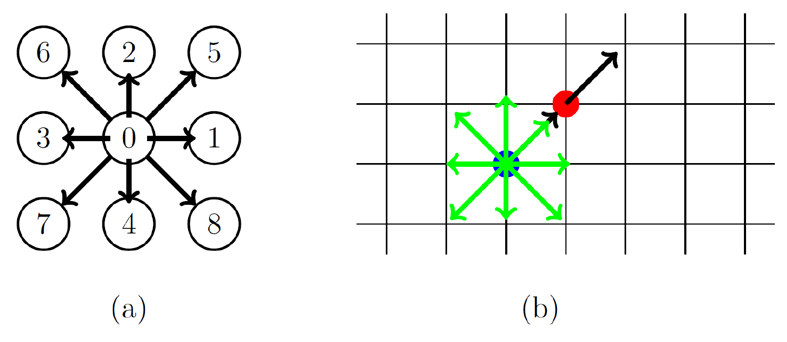
\includegraphics[width=9cm]{d2q9_scheme.png}\\
  (a) Discretization on the velocity space according to D2Q9.\\
  (b) Uniform 2D grid for the discretization in the physical space.\\
  \small{(Material from lecture)}
\end{figure}


\paragraph{Streaming}
As shown in equation~\ref{eq:pdf} streaming and collision are two separate terms.
The collision can be ignored by setting it to zero, i.e. $\left( \frac{\partial f}{\partial t} \right)_{col} \overset{!}{=} 0$.
This simplifies the BTE and implies the movement of particles in the vacuum with no mutual interaction between particles, see equation \ref{eq:streaming}.
\begin{equation}
  \label{eq:streaming}
  \begin{aligned}
    f_{i}(r+c_{i} \nabla t,t+\nabla t)=f_{i}(r,t)
  \end{aligned}
\end{equation}
The code wise implementation of a streaming function on a 2D lattice is shown in listing \ref{lst:streaming}
\footnote{Throughout I will use the notation $_ixy$ where $i$ is the rolling dimension and x and y are the deminsions of the physical space.}.
\begin{center}
  \begin{lstlisting}[caption=Implementation of the streaming term,label=lst:streaming, basicstyle=\small]
    def stream(f_cxy: np.array) -> np.array:
      for i in range(1, 9):
        f_cxy[i, :, :] = np.roll(f_cxy[i, :, :], 
                                  shift=C_CA[i], 
                                  axis=(0, 1))
      return f_cxy
  \end{lstlisting}
\end{center}
Where $f_{cxy}$ is the PDF and $C \_ CA$ are the discretized velocity directions.

\paragraph{Collision}
The collision term is the \textit{r.h.s} of the BTE \ref{eq:BTE} and represents the interaction between particles.
It is a complicated two particle scattering integral but can be approximated by a relaxation time approximation $\tau$ so that the PDF locally relaxes to an equilibrium distribution $f_{eq}(r,v,t)$.
The resulting discrete form of the BTE is shown in equation
\begin{equation}
  \label{eq:btw-discrete}
  \begin{aligned}
    f_{i}(r+ \nabla t c_{i},t+\nabla t)=f_{i}(r,t) + \omega \left( f_{i}^{eq}(r,t) - f_{i}(r,t) \right)
  \end{aligned}
\end{equation}
Because of the relaxation the PDF equilibrium is a local one and therefor depends on the local denisty $\rho$ and the local average velocity $u$.

The local denisty is just a summation over the velocities of the PDF, i.e. $\rho(r) = \sum_{i} f_{i}$.
An example implementation is shown in listing \ref{lst:rho}.
\begin{center}
  \begin{lstlisting}[caption=Implementation of the local density,label=lst:rho, basicstyle=\small]
    def local_density(f_cxy: np.array) -> np.array:
      r_xy = np.einsum("cxy -> xy", f_cxy)
      return r_xy
  \end{lstlisting}
\end{center}
The local average velocity is more complicated but effectively it is the summation over the velocity dimensions for each physical dimension divided by the local density.
It is calculated via $u(r)=\frac{1}{\rho (r)} \sum_{i} c_{i}f_{i}(r)$ and respective code is shown in listing \ref{lst:vel}.
\begin{center}
  \begin{lstlisting}[caption=Implementation of the local average velocity.,label=lst:vel, basicstyle=\small]
    def local_avg_velocity(f_cxy: np.array, r_xy: np.array):
      u_aij = np.einsum("ac, cxy->axy", C_CA.T, f_cxy) / r_xy
      return u_aij
  \end{lstlisting}
\end{center}
With this we can define the PDF equilibrium function as in equation \ref{eq:pdf-eq},
\begin{equation}
  \label{eq:pdf-eq}
  \begin{aligned}
    f_{i}^{eq} ( \rho , u ) = w_i \rho \left[ 1+3 c_i * u + \frac{9}{2}(c_i * u )^2 - \frac{3}{2} | u |^2 \right]
  \end{aligned}
\end{equation}
where $w_i$ for a D2Q9 lattice can be defined as follow: $w_i = \left( \frac{4}{9}, \frac{1}{9}, \frac{1}{9}, \frac{1}{9}, \frac{1}{9}, \frac{1}{36}, \frac{1}{36}, \frac{1}{36}, \frac{1}{36} \right)$.
It is important to note that the approximation in the collision term is not always accurate.
But under the assumption that all transport processes occur on a longer time scale it is appropriate to do.

\section{Shear Wave Decay and Kinematic Viscosity}
Shear wave decay describes the amplitude decay of shear waves, elastic waves travelling through the body of an object.

The kinematic viscocity $\nu$ is especially revelant in fluid dynamics and is defined as the ratio of the dynamic viscosity $\mu$ over the density $\rho$ of the fluid, $\nu = \frac{\mu}{\rho}$.

\paragraph{M3.1} We chose an initial distribution of $\rho (r,t_{0}=\rho_{0}+\epsilon \sin \left( \frac{2\pi x}{L_{x}}) \right)$ and $u(r,0)=0$. 
Where $L_{x}$ is the length of the domain in the x direction.

\begin{figure}
  \captionsetup{justification=centering,margin=1cm}
  \includegraphics[scale=0.8]{}
\end{figure}

\centering
\includegraphics[width=0.9\columnwidth]{figs/fig-cell-normal-to-cancer.png}
\caption{Cell development: from normal to cancer. \\Credit: Terese Winslow LLC}
% https://www.cancer.gov/about-cancer/understanding/what-is-cancer
\label{fig:cancer-cell-development}


% .$u(r,0)  ρ(r,0)=\rho_{0}+ \eps \sin \left( \frac{2\pi x}{L_{x}} \right)$



\bibliographystyle{unsrt}
\bibliography{biblio}
% \bibliography{"/home/joe/repos/pylbm/milestones/final/biblio.bib"}

\end{document}
